\section{Motor controller} \label{sec:motor-controller-imp} 
This section describes the implemented motor controller. As described in \secref{sec:design-motor-controller}, the motor controller repeatedly gets the current amount of steps from the motors and helps the robot drive more accurately. The motor controller makes sure that the robot will drive a certain distance precisely, as well as rotating a certain angle precisely. Furthermore, the implemented speed adjuster will keep the robot driving reliably and compensate for the variety in friction on different surfaces and the motors difference.

The motor controller is implemented using logical expressions in an IF-THEN relationship, usually in the form IF <logical expression> THEN <logical expression>. It can be described using propositional logic. The robot uses a knowledge base to determine what is true about the world, or in this case, about the motors. The motor controller observes the world through the input from the motors and makes decisions on how to change the speed of the motors, based on these observations.

\subsection{Propositional logic}
The propositional logic described below is for moving forward and backwards. The rotation controller is omitted, since it functions alike, though with directional changes. The implemented motor controller is split into the two goals, as described in \secref{sec:design-motor-controller}. 

\equref{eq:motorsteps} shows variables, which contains the values returned from the motors. \equref{eq:motorpower} shows the variables, that gives information to the motors, about what power they should run at. \equref{eq:targetsteps} shows the variable that contains the number of steps, that the \projname{} must reach, along with the error margin and variables to hold the adjusted min/max values.
\begin{equation} \label{eq:motorsteps}
\begin{split} 
& motor\_l\_steps \\
& motor\_r\_steps
\end{split}
\end{equation}
\begin{equation} \label{eq:motorpower}
\begin{split}
& motor\_l\_power \\
& motor\_r\_power
\end{split}
\end{equation}
\begin{equation} \label{eq:targetsteps}
\begin{split}
& target\_steps \\
& min\_steps \\
& max\_steps \\
& error\_margin
\end{split}
\end{equation}
It is worth noting that these variables are not boolean values, but are represented as integers. They are used to determine if speed adjusting is needed and what the desired number of steps to drive are. The described variables are used for either the speed adjuster or for the move controller. 


\subsection{Speed adjuster knowledge base}
If speed adjusting was not done continuously, no checks would be made to ensure that the motors are running equally fast. This would result in a robot that would have trouble driving straight. Thus, speed adjusting is performed when one motor is ahead or behind the other motor. This is measured in the amount of steps the motors have driven. This is illustrated in the propositions in \equref{eq:motorxahead}.
\begin{equation} \label{eq:motorxahead}
\begin{split}
& motor\_r\_ahead \leftarrow motor\_l\_steps~<~motor\_r\_steps \\
& motor\_l\_ahead \leftarrow motor\_l\_steps~>~motor\_r\_steps
\end{split}
\end{equation}
The atomic proposition $motor\_r\_ahead$, illustrates if the right motor is ahead, in terms of steps. If $motor\_r\_ahead$ is true the motor controller adjusts the motor speed, such that the left motor catches up. Same principle goes for $motor\_l\_ahead$ with adjustments to ensure that the right motor catches up. 

\equref{eq:moving-forward-and-backward} is used to determine which direction the \projname{} is moving. Based on the motor power values, it is determined whether the \projname{} is driving forward or backwards. Note that the gearing makes negative power values result in the \projname{} moving forward. 
\begin{equation} \label{eq:moving-forward-and-backward}
\begin{split}
& moving\_forward \leftarrow motor\_l\_power < 0 \land motor\_r\_power < 0 \\
& moving\_backward \leftarrow motor\_l\_power > 0 \land motor\_r\_power > 0 
\end{split}
\end{equation}
Now that a basis has been set for determining the robots direction and determining if speed adjustment is needed, a knowledge base can be set up. The rest of the section describes the actions that the speed adjuster performs, as a set of multiple propositional definite clauses. The set of these definite clauses make up the knowledge base that the speed adjuster utilises. Most of the definite clauses are on the form $a \leftarrow b$, which is also known as a rule. The symbol on the left of the arrow is known as an atomic proposition, or just atom, and on the right is another atomic proposition or a conjunction of atomic propositions. The rest of the definite clauses are just atomic propositions.

By using \equref{eq:motorxahead} and \equref{eq:moving-forward-and-backward}, the definite propositions for the $decrease\_speed$ and $increase\_speed$ can be made. These can be seen in \equref{eq:decrease-increase-speed}. Given knowledge about the direction and which motor is ahead, it can be observed whether or not the speed should be increased, decreased or if no adjusting should be done. 
\begin{equation} \label{eq:decrease-increase-speed}
\begin{split}
& decrease\_speed \leftarrow motor\_l\_ahead \land (moving\_forward \lor moving\_backward) \\
& increase\_speed \leftarrow motor\_r\_ahead \land (moving\_forward \lor moving\_backward) \\
\end{split}
\end{equation}
This leads to the final proposition, $adjust\_speed$, seen in \equref{eq:adjust-speed}. 
\begin{equation} \label{eq:adjust-speed}
adjust\_speed \leftarrow decrease\_speed \lor increase\_speed 
\end{equation}
Using \equref{eq:motorxahead} and \equref{eq:moving-forward-and-backward}, the knowledge base for the speed adjuster has been created. The knowledge base can be seen in \equref{eq:knowledge-base-speed-adjuster}. 
\begin{equation} \label{eq:knowledge-base-speed-adjuster}
\begin{split}
& adjust\_speed \leftarrow decrease\_speed \\
& adjust\_speed \leftarrow increase\_speed \\
& decrease\_speed \leftarrow motor\_l\_ahead \land moving\_forward \\
& decrease\_speed \leftarrow motor\_l\_ahead \land moving\_backward \\
& increase\_speed \leftarrow motor\_r\_ahead \land moving\_forward \\
& increase\_speed \leftarrow motor\_r\_ahead \land moving\_backward \\
& motor\_l\_ahead \\
& motor\_r\_ahead \\
& moving\_forward \\
& moving\_backward
\end{split}
\end{equation}


\subsection{Move controller knowledge base}
Adjusting the speed of the motors is only one part of the motor controller. The following definite clauses describes how the motor controller ensures that the \projname{} drives to the targeted distance precisely and stops. The motor controller does the same for angles to rotate, but as mentioned previously, the propositional logic for this is omitted, because this functions the same way as driving a distance, but with adjusted values.

The propositions in \equref{eq:min-max-steps}, is used to determine if the \projname{} has reached the desired distance, $+/-$ the error margin. 
\begin{equation} \label{eq:min-max-steps}
\begin{split}
& min\_steps \leftarrow (target\_steps~-~error\_margin) \\
& max\_steps \leftarrow (target\_steps~+~error\_margin)
\end{split}
\end{equation}
As with the case of speed adjusting, before setting up the definite clauses, a few other propositions are needed. The proposition seen in \equref{eq:within-error-margin}, determines if the robot is inside the targeted amount of steps, $+/-$ the error margin. The atom $within\_error\_margin$ is true, if either the left or the right motor is inside the accepted margin. It is only necessary to check one of the motors, as the speed adjuster ensures that the motors are within a reasonable amount of steps of each other. 
\begin{equation} \label{eq:within-error-margin}
\begin{split}
within\_error\_margin & \leftarrow (min\_steps~<~motor\_r\_steps \land motor\_r\_steps~<~max\_steps) \\
& \lor (min\_steps~<~motor\_l\_steps \land motor\_l\_steps~<~max\_steps)
\end{split}
\end{equation}
With these propositions set up, the definite clauses for the move controller can be defined. \equref{eq:target-distance-reached} shows the proposition that says whether or not the targeted distance has been reached. 
\begin{equation} \label{eq:target-distance-reached}
target\_distance\_reached \leftarrow within\_error\_margin
\end{equation}
This leads to the definite clause seen in \equref{eq:keep-moving}. This says, that if the target has not been reached, then the \projname{} keeps moving.
\begin{equation} \label{eq:keep-moving}
keep\_moving \leftarrow \lnot target\_distance\_reached
\end{equation}
These has resulted in the knowledge base seen in \equref{eq:knowledge-base-move-controller}. 
\begin{equation} \label{eq:knowledge-base-move-controller}
\begin{split}
& keep\_moving \leftarrow \lnot target\_distance\_reached \\
& target\_distance\_reached \leftarrow within\_error\_margin \\
& within\_error\_margin
\end{split}
\end{equation}


\subsection{Querying the knowledge bases}
With these knowledge bases, the motor controller could be queried at any point about what is true in the world regarding the motors. The knowledge base is updated live as data are received from the motors. A query could for example be, ``ask $target\_distance\_reached$''. The motor controller would check the knowledge base and return an answer. This is essentially what the motor controller is doing in practice, repeatedly checking if some conditions have been met.

This can be shown in terms of proofs. A proof is a way of demonstrating that a proposition logically follows from a knowledge base. Given a proof procedure, KB $\vdash p$ means $p$ can be proven from knowledge base KB. These proofs can be illustrated using proof trees. In \figref{fig:speed-tree} and \figref{fig:move-tree} a potential query for each of the knowledge bases are proved.
\begin{figure}[H]
     \center{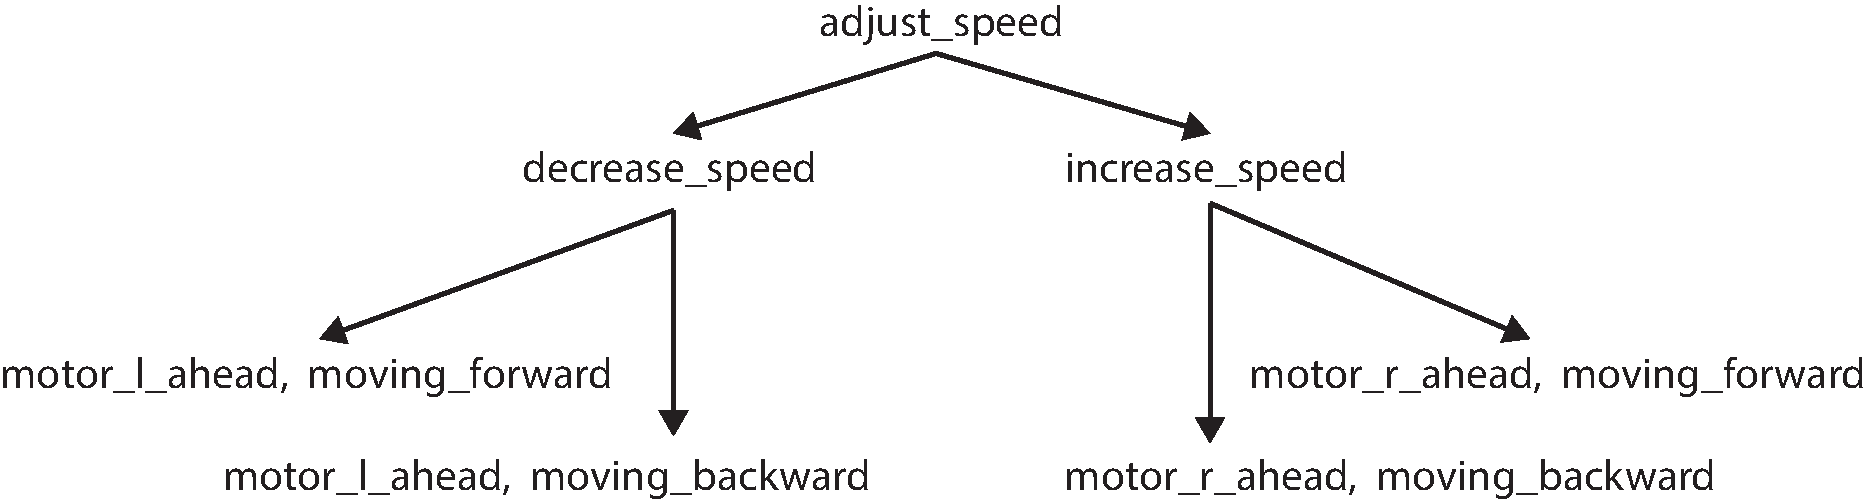
\includegraphics[width=\textwidth]
     {graphics/SpeedTree.pdf}}
     \caption{\label{fig:speed-tree} Proof tree for the query, ``ask $adjust\_speed$''}
\end{figure}
In \figref{fig:speed-tree} it is asked if the speed should be adjusted. To prove $adjust\_speed$ the tree can be traversed using a top-down procedure. To determine if $adjust\_speed$ is true, $decrease\_speed$ and $increase\_speed$ has to be checked, and if either of these are true, then the $adjust\_speed$ must be true. But to determine if these are true, further propositions have to be checked. This must be done until the knowledge needed is provided, which is gained from atoms that the knowledge base knows are true.
\begin{figure}[H]
     \center{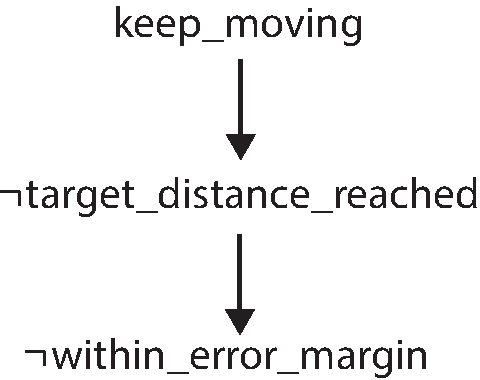
\includegraphics[scale=0.5]
     {graphics/MoveTree.pdf}}
     \caption{\label{fig:move-tree} Proof tree for the query, ``ask $keep\_moving$''}
\end{figure}
\figref{fig:move-tree} is determining if the robot should keep moving, based on whether or not the target distance has been reached. As long as $within\_error\_margin$ is false, the $target\_distance\_reached$ is also false which leads to $keep\_moving$ being true. This means that as long as the robot is not within the error margin, the target distance has not been reached and the robot should keep moving.
